% Version 3 December 2023
% See section 11 of the User Manual for version history
%
%%%%%%%%%%%%%%%%%%%%%%%%%%%%%%%%%%%%%%%%%%%%%%%%%%%%%%%%%%%%%%%%%%%%%%
%%                                                                 %%
%% Please do not use \input{...} to include other tex files.       %%
%% Submit your LaTeX manuscript as one .tex document.              %%
%%                                                                 %%
%% All additional figures and files should be attached             %%
%% separately and not embedded in the \TeX\ document itself.       %%
%%                                                                 %%
%%%%%%%%%%%%%%%%%%%%%%%%%%%%%%%%%%%%%%%%%%%%%%%%%%%%%%%%%%%%%%%%%%%%%

%%\documentclass[referee,sn-basic]{sn-jnl}% referee option is meant for double line spacing

%%=======================================================%%
%% to print line numbers in the margin use lineno option %%
%%=======================================================%%

%%\documentclass[lineno,sn-basic]{sn-jnl}% Basic Springer Nature Reference Style/Chemistry Reference Style

%%======================================================%%
%% to compile with pdflatex/xelatex use pdflatex option %%
%%======================================================%%

%%\documentclass[pdflatex,sn-basic]{sn-jnl}% Basic Springer Nature Reference Style/Chemistry Reference Style

%%Note: the following reference styles support Namedate and Numbered referencing. By default the style follows the most common style. To switch between the options you can add or remove “Numbered” in the optional parenthesis.\\

%%The option is available for: sn-basic.bst, sn-vancouver.bst, sn-chicago.bst%

%%\documentclass[pdflatex,sn-nature]{sn-jnl}% Style for submissions to Nature Portfolio journals
%%\documentclass[pdflatex,sn-basic]{sn-jnl}% Basic Springer Nature Reference Style/Chemistry Reference Style
\documentclass[pdflatex, sn-mathphys-num, lineno]{sn-jnl}% Math and Physical Sciences Numbered Reference Style
%%\documentclass[pdflatex,sn-mathphys-ay]{sn-jnl}% Math and Physical Sciences Author Year Reference Style
%%\documentclass[pdflatex,sn-aps]{sn-jnl}% American Physical Society (APS) Reference Style
%%\documentclass[pdflatex,sn-vancouver,Numbered]{sn-jnl}% Vancouver Reference Style
%%\documentclass[pdflatex,sn-apa]{sn-jnl}% APA Reference Style
%%\documentclass[pdflatex,sn-chicago]{sn-jnl}% Chicago-based Humanities Reference Style

%%%% Standard Packages
%% additional latex packages if required can be included here>
\usepackage{graphicx}%
\usepackage{multirow}%
\usepackage{amsmath,amssymb,amsfonts}%
\usepackage{amsthm}%
\usepackage{mathrsfs}%
\usepackage[title]{appendix}%
\usepackage{xcolor}%
\usepackage{textcomp}%
\usepackage{manyfoot}%
\usepackage{booktabs}%
\usepackage{algorithm}%
\usepackage{algorithmicx}%
\usepackage{algpseudocode}%
\usepackage{listings}%

\usepackage{xspace}
\usepackage{standalone}

%% my package
\usepackage[detect-all=true]{siunitx}
\sisetup{
    scientific-notation=false,
    round-mode = places,
    round-precision = 2
}

\usepackage[acronym, automake, style=index, shortcuts]{glossaries-extra}

\setabbreviationstyle[acronym]{long-short}

% define glossaries
\makeglossaries
\newacronym{blat}{BLAT}{BLAST-like alignment tool}
\newacronym{llm}{LLM}{Large language model}
\newacronym{hmm}{HMM}{Hidden Markov Model}
\newacronym{gpu}{GPU}{Graphics Processing Unit}
\newacronym{drs}{DRS}{NanoPore direct RNA sequencing}
\newacronym{bert}{BERT}{Bidirectional Encoder Representations from Transformers}
\newacronym{gpt}{GPT}{Generative Pre-trained Transformer}

\newacronym{ide}{IDE}{Integrated Development Environment}
\newacronym{cd}{CD}{Continuous Development}
\newacronym{ucsc}{UCSC}{UCSC Genome Browser}
\newacronym{glm}{GLM}{Genomic Language Model}
\newacronym{lcglm}{LCGLM}{Long-Context Genomic Language Model}
\newacronym{snp}{SNP}{single nucleotide polymorphism}
\newacronym{fm}{FM}{Foundational Model}
\newacronym{nlp}{NLP}{natural language processing}

\newacronym{tp}{TP}{true positive}
\newacronym{fp}{FP}{false positive}
\newacronym{fn}{FN}{false negative}

% define macros
% chopper = DeepChopper
\newcommand{\chopper}{DeepChopper\xspace}

\newcommand{\figref}[2]{Figure~\hyperref[#1]{\ref*{#1}#2}}

%%%%%=============================================================================%%%%
%%%%  Remarks: This template is provided to aid authors with the preparation
%%%%  of original research articles intended for submission to journals published
%%%%  by Springer Nature. The guidance has been prepared in partnership with
%%%%  production teams to conform to Springer Nature technical requirements.
%%%%  Editorial and presentation requirements differ among journal portfolios and
%%%%  research disciplines. You may find sections in this template are irrelevant
%%%%  to your work and are empowered to omit any such section if allowed by the
%%%%  journal you intend to submit to. The submission guidelines and policies
%%%%  of the journal take precedence. A detailed User Manual is available in the
%%%%  template package for technical guidance.
%%%%%=============================================================================%%%%

%% as per the requirement new theorem styles can be included as shown below
\theoremstyle{thmstyleone}%
\newtheorem{theorem}{Theorem}%  meant for continuous numbers
%%\newtheorem{theorem}{Theorem}[section]% meant for sectionwise numbers
%% optional argument [theorem] produces theorem numbering sequence instead of independent numbers for Proposition
\newtheorem{proposition}[theorem]{Proposition}%
%%\newtheorem{proposition}{Proposition}% to get separate numbers for theorem and proposition etc.

\theoremstyle{thmstyletwo}%
\newtheorem{example}{Example}%
\newtheorem{remark}{Remark}%

\theoremstyle{thmstylethree}%
\newtheorem{definition}{Definition}%

\raggedbottom
\unnumbered% uncomment this for unnumbered level heads

\begin{document}

\title[Article Title]{Language models identify chimeric artificial read in NanoPore direct-RNA sequencing data.}

%%=============================================================%%
%% GivenName	-> \fnm{Joergen W.}
%% Particle	-> \spfx{van der} -> surname prefix
%% FamilyName	-> \sur{Ploeg}
%% Suffix	-> \sfx{IV}
%% \author*[1,2]{\fnm{Joergen W.} \spfx{van der} \sur{Ploeg}
%%  \sfx{IV}}\email{iauthor@gmail.com}
%%=============================================================%%

\author[1]{\fnm{Yangyang} \sur{Li}}\email{yangyang.li@northwestern.edu}
\equalcont{These authors contributed equally to this work.}

% \author*[1,2]{\fnm{First} \sur{Author}}\email{iauthor@gmail.com}
\author[1]{\fnm{Tingyou} \sur{Wang}}\email{tingyou.wang@northwestern.edu}
\equalcont{These authors contributed equally to this work.}

\author[1]{\fnm{Qingxiang} \sur{Guo}}\email{qingxiang.guo@northwestern.edu}
\author*[1,2]{\fnm{Rendong} \sur{Yang}}\email{rendong.yang@northwestern.edu}

\affil[1]{\orgdiv{Department of Urology}, \orgname{Northwestern University Feinberg School of Medicine}, \orgaddress{\street{303 E Superior St}, \city{Chicago}, \postcode{60611}, \state{IL}, \country{USA}}}
\affil[2]{\orgdiv{Robert H. Lurie Comprehensive Cancer Center}, \orgname{Northwestern University Feinberg School of Medicine}, \orgaddress{\street{675 N St Clair St}, \city{Chicago}, \postcode{60611}, \state{IL}, \country{USA}}}

% \author[1,2]{\fnm{Third} \sur{Author}}\email{iiiauthor@gmail.com}
% \equalcont{These authors contributed equally to this work.}

% \affil*[1]{\orgdiv{Department}, \orgname{Organization}, \orgaddress{\street{Street}, \city{City}, \postcode{100190}, \state{State}, \country{Country}}}
% \affil[2]{\orgdiv{Department}, \orgname{Organization}, \orgaddress{\street{Street}, \city{City}, \postcode{10587}, \state{State}, \country{Country}}}
% \affil[3]{\orgdiv{Department}, \orgname{Organization}, \orgaddress{\street{Street}, \city{City}, \postcode{610101}, \state{State}, \country{Country}}}

%%==================================%%
%% Sample for unstructured abstract %%
%%==================================%%

\abstract{
	\glspl{llm} have revolutionized natural language processing and are now poised to transform biological sequence analysis.
	This study explores the application of \glspl{llm} to \gls{drs} data, focusing on predicting adapters.
	Our results demonstrate that \glspl{llm} can effectively handle long contexts in biological sequences, providing accurate and efficient predictions.
	This showcases the potential for broader applications of \glspl{llm} in genomics and transcriptomics, offering a powerful tool for the biotechnology field.}

\maketitle
\section{Main}\label{sec1}

%Long Context Strategies in Genomic

%To achieve longer context, genomic models have relied on two strategies: i. tokenization and ii. dilation and downsampling.
%Tokenization is a necessary step in masked language modeling (MLM) with bidirectional Transformer architectures (BERT) (Devlin et al., 2018), a common model in genomics.
%These tokenizers use fixed k-mers (short overlapping sequences of length k) or frequency-based byte pair encoding (BPE), that attempt to aggregate DNA into meaningful units (Ji et al., 2021; Zaheer et al., 2020).
%Consequently, these aggregation techniques create large new vocabularies (compared to the natural vocabulary of 4 nucleotides) that are less generalizable (Tay et al., 2021).
%The second strategy uses dilated convolutions and downsampling, both of which essentially average or skip elements between weights (Fournier et al., 2021).
%A canonical example is the Enformer, which uses dilation and downsampling to reach context lengths of 100k nucleotides to predict gene expression tracks (Avsec et al., 2021).
%Common across tokenization, dilation, and downsampling is the sacrifice of single nucleotide resolution to reach longer context.


% Outline
% 1. Sequencing history
% 2. Genomics LLM history
% 3. Challenges of LLM / efficiency of transformer and improvements (hyena)
% 3.1 long range
% 3.2 single nucleotide resolution
% 4. Cons of drs
% 5. Our method
% 6. Results
% 7. Conclusion

The advent of high-throughput sequencing technologies has revolutionized genomics, providing unprecedented insights into the genetic underpinnings of biological processes.
Among these technologies, Oxford \gls{drs} stands out as a powerful tool for sequencing full-length RNA molecules, with the unique advantage of preserving native RNA modifications.
However, despite its transformative potential, \gls{drs} faces a significant challenge: the generation of chimeric artificial reads, where fragments of distinct RNA molecules are incorrectly joined together.
Accurately identifying these chimeric sequences is critical, as their presence compromises data quality and hinders downstream analyses, including transcriptome assembly, quantification, and gene fusion detection.

In recent years, \glspl{llm} have made remarkable strides across various fields, including \gls{nlp} and, more recently, genomics.
Genomic \glspl{llm}, trained on vast amounts of sequencing data, have demonstrated an unprecedented ability to capture complex sequence patterns and predict functional elements~\cite{nguyen2024hyenadna, dalla2023nucleotide, zhou2023dnabert2}.
However, their application to genomics is not without challenges, particularly when addressing the long-range dependencies inherent in sequencing data and achieving single-nucleotide resolution.


Traditional methods  often struggle with the intricacies of long RNA sequences, leading to errors and inefficiencies.
Transformers, which form the backbone of most \gls{llm}, excel at modeling long-range dependencies, but their quadratic scaling with sequence length poses efficiency challenges in processing genomic data~\cite{tay2022efficient}.
While transformer-based genomic models can handle sequences up to 4k tokens, this represents less than $0.001\%$ of the human genome, significantly limiting their capacity to model long-range interactions in DNA~\cite{dalla2023nucleotide, zhou2023dnabert2, ji2021dnabert}.
Although innovations like the Hyena architecture have optimized long-range attention mechanisms, offering improved efficiency and scalability, single-nucleotide resolution remains elusive—a crucial aspect for understanding the complexities of biological sequences, where subtle variations can profoundly impact protein function~\cite{poli2023hyena, nguyen2024hyenadna}.

Despite advances in \gls{drs}, the technology remains susceptible to the formation of chimeric reads, particularly in long-read sequencing, complicating the accurate interpretation of results.
Addressing this issue is critical for ensuring the reliability of DRS data in both research and clinical applications.

In response to these challenges, we developed \chopper, a language model specifically tailored for biological sequences.
Leveraging state-of-the-art \gls{llm} architectures and training paradigms, our model was trained on extensive \gls{drs} datasets to predict artificial sequences with high accuracy.
Unlike traditional methods, which rely on tokenizers or fixed k-mers and often lose single-nucleotide resolution, \chopper treats biological sequences as a form of language, capturing the underlying biological grammar and enabling it to predict artificial sequences embedded within long reads.

Traditional hard clipping methods can only predict terminal adapters—artificial sequences at the ends of reads.
In contrast, \chopper excels at identifying chimeric reads formed by artificial sequences located in the middle of reads.
Our model significantly outperforms traditional algorithms, particularly in handling the length and variability inherent in RNA sequences.

Our findings demonstrate that DeepChopper can effectively parse vast amounts of sequencing data, identifying artificial sequences with remarkable accuracy.
This capability is crucial for improving the overall quality of sequencing data and ensuring reliable downstream analyses.
By successfully predicting artificial sequences in \gls{drs} data, we illustrate the potential of \glspl{llm} to enhance the accuracy and efficiency of biological sequence analysis in long contexts.
This study, exemplified by \chopper, paves the way for broader applications of \glspl{llm} in understanding and interpreting the vast complexities of genomic information.


% Result


%Model Architecture Overview (Fig 1A)

\figref{fig:f1}{a} provides an overview of the \chopper model architecture, highlighting its key components designed for the detection of chimeric reads in \gls{drs} data.
The model employs a HyenaDNA as Feature Extactor, incorporating advanced tokenization and sequence quality assessment mechanisms to handle long-range dependencies inherent in sequencing data~\cite{nguyen2024hyenadna}.
The architecture is specifically tailored to biological sequences, enabling it to differentiate between true biological reads and chimeric artifacts with high accuracy.
By leveraging residual connections and long-range attention mechanisms, \chopper is optimized for processing large volumes of sequencing data efficiently, making it a powerful tool for improving data quality in genomic research. This foundational architecture underpins the superior performance of \chopper (\figref{fig:f1}{a}).


% Analysis of Predicted Artifact Lengths

The distribution of the lengths of predicted artifacts revealed that \chopper is particularly effective at identifying artifacts within a critical length range, which is often associated with chimeric reads.
The frequency analysis indicated that the majority of the artifacts detected by \chopper were shorter than 250 base pairs, a range where traditional methods tend to struggle due to the ambiguous nature of such sequences (\figref{fig:f1}{b}).

% Positional Bias in Chimeric Read Prediction

An interesting pattern emerged when analyzing the relative positions of the predicted chimeric artifacts.
\chopper showed a consistent ability to identify chimeric sequences not only at the ends of reads (typically addressed by traditional clipping methods) but also those embedded within the middle of long reads (\figref{fig:f1}{c}).
This capability is particularly crucial for long-read sequencing platforms, where chimeric reads often appear in internal regions, leading to significant errors in downstream analyses.

% The number of prediction intervals

We analyzed the number of prediction intervals identified by \chopper in VCaP 002.
A prediction interval is defined as a contiguous sequence within a read where the model predicts the presence of artificial sequences.
The number of such intervals provides insight into the frequency and distribution of artificial sequences in every chimeric read.
Our results revealed a distinct distribution pattern in the number of prediction intervals, with the majority of reads containing between 2 and 5 intervals (\figref{fig:f1}{d}).
This finding suggests that chimeric artifacts are often not confined to a single region within a read but are spread across multiple locations.
The ability of \chopper to detect multiple prediction intervals within the same read highlights its sensitivity in identifying fragmented chimeric sequences that might be missed by traditional methods.
By capturing multiple intervals, \chopper provides a more detailed and accurate characterization of these artifacts, which is crucial for downstream applications such as transcriptome assembly and gene fusion detection.

% Chimeric Read Detection Across Sequencing Platforms Fig 1 E

We observed that \chopper consistently outperformed Dorado, both with and without trimming, in detecting chimeric reads in the VCaP 002 dataset.
\chopper achieved a 91\% reduction in the total count of chimeric reads, highlighting its effectiveness in minimizing these artifacts.
To further validate this capability, we used ONT PCR cDNA data (\figref{fig:f1}{e}).
The results showed that \chopper identified significantly fewer unsupported reads compared to baseline methods, indicating its superior accuracy in filtering out chimeric artifacts.
Notably, \chopper reduced the number of unsupported reads by nearly 94\% and achieved  supporting rate 47\% compared 5\%, demonstrating its exceptional ability to distinguish true biological sequences from chimeric constructs (\figref{fig:f1}{e}).

% Base Quality of Detected Artificial Sequences (Fig 1F)
We analyzed the base quality of artificial sequences detected by \chopper, as identified in \figref{fig:f1}{e}.
The base quality score is a critical metric for assessing the reliability of sequencing data, with higher scores indicating greater confidence in the accuracy of the detected bases.
The results revealed that the artificial sequences identified by \chopper consistently exhibited lower base quality scores compared to true biological sequences (\figref{fig:f1}{f}).
This finding underscores the model's ability to differentiate between high-confidence true reads and low-confidence artificial sequences.
Specifically, \chopper effectively flagged sequences with diminished base quality, aligning with the expected profile of chimeric or erroneous reads.
The clear distinction in base quality between supported and unsupported reads further validates \chopper's accuracy in identifying and filtering out artificial sequences.
By maintaining a high level of precision in detecting these lower-quality sequences, \chopper enhances the overall integrity of the sequencing data, ensuring that downstream analyses are based on more accurate and reliable reads.


% BLAT Identity of Detected Artificial Sequences (Fig 1G)
\figref{fig:f1}{g} evaluates the \gls{blat} identity of the artificial sequences detected by \chopper, as identified in \figref{fig:f1}{e}.
\gls{blat} identity measures the similarity of the sequences to known reference sequences, with lower identity scores indicating potential chimeric or erroneous reads.
The results show that the artificial sequences identified by \chopper consistently have lower BLAT identity compared to true biological sequences.
This finding highlights the model's proficiency in detecting sequences that diverge from expected reference sequences, further confirming their artificial nature.

% Chimeric Read Detection Across Multiple Samples (Fig 1H)
\figref{fig:f1}{h} presents the results of chimeric read detection across five different samples including A549, HCT116, HepG2, K562 and MCF7, mirroring the analysis shown in \figref{fig:f1}{e}.
Each subfigure  illustrates the performance of \chopper in identifying and filtering out chimeric reads in different datasets.
Consistently across all samples, \chopper significantly reduced the number of chimeric reads compared to baseline methods ( 62\% - 84\%), demonstrating its robustness and reliability in diverse sequencing contexts.
The supporting rate of Dorado with trimming was 8\% to 19\%, while \chopper achieved a supporting rate from 43\% to 55\%.
The reduction rates were comparable to those observed in \figref{fig:f1}{e}, further validating DeepChopper’s superior capability to distinguish true biological sequences from chimeric constructs across various sample types.
These consistent results across multiple samples underscore the model's broad applicability and effectiveness.

% Supporting Read Analysis Across Multiple Datasets (Fig 1I)
\figref{fig:f1}{i} focuses on the analysis of supporting reads in the wtc11 sample, utilizing five different datasets: ONT PCR cDNA, ONT CapTrap, ONT R2C2, PacBio (PB) cDNA, and PB CapTrap.
Our model reduce the number of chimeric reads by 54\% compare Dorado with trim for wtc11.
Each subfigure illustrates the proportion of supporting reads (51\% to 66\%) detected by \chopper across these datasets, and the rate of supporting reads of Dorado with trimming (26\% to 37\%).
Despite the variation in sequencing platforms and protocols, \chopper consistently achieved high support rates in identifying true biological sequences while effectively filtering out chimeric reads.
The results demonstrate the model's versatility and accuracy across diverse datasets, confirming its capability to maintain data integrity across different sequencing conditions.
The consistency of these findings across the multiple datasets reinforces the reliability of \chopper in enhancing the quality of nanopore direct RNA sequencing data.

\begin{figure}[!h]
	\includegraphics[height=0.78\columnwidth]{figures/finals/figure1}
    \caption{{\bf  Detection and Analysis of Chimeric Reads in Nanopore Direct RNA Sequencing Data Using \chopper.} (a) Overview of the \chopper model architecture, highlighting key components such as tokenization, sequence quality assessment, and prediction blocks. The model is designed to identify artificial sequences by leveraging advanced transformer-based techniques. (b) Distribution of the lengths of predicted artifacts detected by DeepChopper in the VCaP 002 dataset. (c) Analysis of the relative positions of prediction artifacts within the VCaP 002 dataset.  (d) Number of prediction intervals detected by DeepChopper in the VCaP 002 dataset. (e) Chimeric read detection performance of DeepChopper compared to Dorado (with and without trimming) in the VCaP 002 dataset. The blue bars represent chimeric reads unsupported by ONT PCR cDNA, while the red bars indicate chimeric reads supported by ONT PCR cDNA.  (f) Base quality scores of the artificial sequences identified by DeepChopper. The figure includes three background colors representing different levels of base quality: green for high base quality, yellow for medium base quality, and red for low base quality. (g) BLAT identity analysis of the artificial sequences detected by DeepChopper. (h) Chimeric read detection across multiple samples, including VCaP 002, A549, HCT116, K562, and MCF7. In each sample, the blue bars represent chimeric reads unsupported by ONT PCR cDNA, while the red bars indicate chimeric reads supported by ONT PCR cDNA. (i)  Supporting read analysis for wtc11, calculated supporting rate using five different datasets: ONT PCR cDNA, ONT CapTrap, ONT R2C2, PacBio (PB) cDNA, and PB CapTrap. The blue bars represent chimeric unsupported reads, while the red bars indicate  supported chimeric reads}
	\label{fig:f1}
\end{figure}


These findings suggest that \glspl{llm} can effectively handle the complexity and variability of biological sequences, making them a valuable tool for improving the accuracy of \gls{drs}.
This not only enhances the quality of sequencing data but also opens up new possibilities for the application of language models in other areas of genomics and transcriptomics.



In the VCaP cell line, genes in the FP group exhibited significantly higher expression levels compared to reference genes (\(\textrm{p-value} < 2.2 \times 10^{-16}\)) (\figref{fig:f2}{A}), despite displaying similar gene lengths (\figref{fig:f2}{B}).
To further explore the functional roles of FP group genes, we conducted Gene Ontology (GO) enrichment analysis across six cell lines—VCaP, A549, K562, HepG2, MCF7, and HCT116 (Figure S2A-S2F).
Interestingly, despite distinct input gene sets, these cell lines converged on common housekeeping functions, including translation, ribosomal small subunit biogenesis, and rRNA processing, etc. (\figref{fig:f2}{C}).

Our study demonstrates the potential of large language models in biological sequence analysis, particularly in the context of \gls{drs}.
By accurately predicting adapter sequences,  \glspl{llm} can significantly improve the quality and reliability of sequencing data.
This showcases the broader applicability of language models in handling complex biological data, paving the way for advancements in genomics and transcriptomics.
Future research can explore additional applications and further optimize these models for specific biological tasks, solidifying their role in biotechnology.

\begin{figure}[!h]
	\includegraphics[height=1.2\columnwidth]{figures/finals/figure2}
	\caption{\bf This is figure 2.}
	\label{fig:f2}
\end{figure}

\section{Methods}\label{sec:methods}

\subsection{Cell culture}

VCaP cell lines were obtained from the American Type Culture Collection (ATCC) and cultured under sterile conditions to maintain optimal growth and viability.
The cells were grown in Dulbecco's Modified Eagle Medium (DMEM, high glucose; Gibco, Cat\# 11-965-092) supplemented with 10\% fetal bovine serum (FBS Opti-Gold, Performance Enhanced, US Origin; Gendepot, Cat\# F0900-050) to provide essential growth factors.
In addition, the culture medium was enriched with \SI{5}{\ml} of 100 mM \( 100\times \) Sodium Pyruvate (Gendepot, Cat\# CA017-010) to support cellular metabolism and \SI{5}{\ml} of Antibiotics-Antimycotics (\( 100\times \)) (Gendepot, Cat\# CA002-010) to prevent microbial contamination.
Cells were cultured in \SI{100}{\mm} cell culture treated dishes (Thermo Fisher Scientific, Cat\# 12-556-002) and incubated at \SI{37}{\degreeCelsius} in a humidified atmosphere containing 5\% CO2, with media changes performed every 72 hours to ensure nutrient availability and waste removal.
Cell confluency was regularly monitored, and subculturing was done before reaching 80\% confluency to maintain healthy growth conditions and prevent over-confluence stress.

\subsection{RNA extraction and quantification}

Total RNA was extracted using the miRNeasy Mini Kit (Qiagen, Cat\# 217004) according to the protocol of manufacturer.
The quality and concentration of RNA were assessed using an Agilent 2100 Bioanalyzer.
Poly(A)+ RNA was then enriched from the total RNA using the Dynabeads\textsuperscript{tm} mRNA Purification Kit (Invitrogen, Cat\# 65001), which utilizes oligo (dT) beads for selective mRNA binding.
The mRNA was quantified using a Qubit 4 fluorometer and a Qubit RNA HS Assay Kit (Thermo Fisher Scientific, Cat\# Q32852).
The mRNA preparations were either immediately used to prepare a sequencing library or frozen and stored at \SI{-80}{\degreeCelsius} until further use.

\subsection{Nanopore sequencing}

We performed nanopore sequencing of the enriched mRNA using two different chemistries: the DNA-nanopore (R9 chemistry; RNA002 kit) and the RNA-nanopore chemistry (RNA chemistry; RNA004 kit).
For the RNA002 library, \SI{1}{\micro\gram} of poly(A)+ RNA was used as input for library preparation using the Direct RNA Sequencing Kit (SQK-RNA002, Oxford Nanopore Technologies) following the manufacturer's instructions.
Direct RNA nanopore sequencing employs a reverse transcriptase adapter (RTA) that typically binds to the poly(A) tails of messenger RNA (mRNA); subsequently, a sequencing adapter is ligated to the RTA, which guides the mRNA through the nanopore for sequencing.
The prepared library was loaded onto a MinION flow cell (FLO-MIN106) and sequenced for 48 hours using the Oxford Nanopore MinION device.
For the RNA004 library, 300 ng of poly(A)+ RNA was used as input for library preparation using the Direct RNA Sequencing Kit (SQK-RNA004, Oxford Nanopore Technologies) according to the protocol of manufacturer.
The library was then loaded onto a PromethION RNA Flow Cell (FLO-PRO004RA) and sequenced on the Oxford Nanopore PromethION device for 72 hours.


\subsection{Training data preparation}\label{ssec:data}


We obtained ONT directRNA FAST5 data from the SG-Nex project, encompassing six cell lines (HEK293T, A549, K562, HepG2, MCF7, and HCT116).
FASTQ files were generated using Dorado (version 0.5.2) with adapter trimming disabled (``--no-trim'').
Reads were then aligned to the human reference genome (hg38) using minimap2 (version 2.24) with optimized ONT directRNA parameters (``-ax splice -uf -k14'').
During the adapter extraction step, we selected primary alignments that lacked supplementary alignments; the 3 soft-clipped regions of these alignments were treated as adapter sequences, while the aligned portions were considered non-adapter sequences.
To create artificial chimeric reads for model training, we randomly selected two non-adapter sequences from the repository and one adapter sequence from the adapter repository, repeating this process multiple times to generate the chimeric dataset.



The raw sequencing data were obtained in fast5 format from the RNA002 run and pod5 format from the RNA004 run.
For base calling, we used Dorado (v0.7.1) for both datasets~\cite{dorado2023}.
The RNA002 data were processed using the rna002\_70bps\_hac model, while the RNA004 data were basecalled using the rna004\_130bps\_hac model.
After base calling, we removed short reads (\( < 50 \) bases) using SeqKit (v2.4.0).
The resulting fastq files were then aligned to the human reference genome (GRCh38) using Minimap2 (v2.26) with the \textit{-ax splice -uf -k7} configuration for direct RNA reads~\cite{li2018minimap2}.
We converted the resulting sam files to bam files, indexed, and sorted them using SAMtools (v1.17) to obtain the genome coverage distribution~\cite{li2009sequence}.

The dataset for this study comprised publicly available \gls{drs} data from the SG-NEx data, which was accessed on 2024 at \url{registry.opendata.aws/sg-nex-data}~\cite{chen2021systematic}.
The SG-NEx data contain six samples including A549, HCT116, HepG2, K562, and MCF7.
We obtain artificial sequence in terms of soft clip from alignment data.
The dataset consist of positive and negative data, in which there is no artificial sequence.
The positive data include terminal and  internal adapters with ratio of \( 1:1 \) respectively.
The ratio between positive data  and negative data is \( 9:1 \).
Totally, we generated \num{600000} data points for training.
The dataset was split into training, validation, and test sets with ration \num{0.8}, \num{0.1}, and \num{0.1} respectively.
Then, we have \num{480000} data points for training, \num{60000} for validation, and \num{60000} million for test.

\subsection{Language model architecture}\label{ssec:lm}

We formulate the problem as a token classification task, where the model predicts the region of artificial sequences.
For each token, the model predicts two classes of artificial sequences: positive and negative, which means the token is or is not in artificial sequences.

We design the model for token classification task, which means the model is able to predict the region of artificial sequences.
We adapted a genomics \gls{fm} HyenaDNA as components of model, which is used to conduct feature extraction, and help us better understand the biological sequences~\cite{nguyen2024hyenadna}.
Following the feature extractor, we add a quality block to combine quality of the input sequence to predict output precisely.
The quality block includes a bulk of dense and residual connection.
The quality block accepts the quality of the input sequence and the extracted features from sequences.
Then, a classification head is used to predict probability of artificial sequence for every token (Figure~\ref{fig:f1}).
The model was trained to predict  artificial sequences based on the contextual information present in the biological sequences.

\subsection{Model training}\label{ssec:training}

\textit{Sequence tokenization.} We used a tokenization strategy that converts the biological sequences into tokens at the single nucleotide level.
The tokens contain \emph{A}, \emph{C}, \emph{G}, \emph{T} and \emph{N} as the basic units, allowing the model to capture the fine-grained details of the sequences.

The model was trained using supervised learning, with sequences annotated for artificial sequences.
Training was conducted on a high-performance computing cluster, utilizing two A100 \glspl{gpu} to expedite the process.
The batch size was \num{64}, validation was performed every \num{20000} steps, and we selected the model with the highest validation F1 score for the base prediction task.
The Adam optimizer was used for training with default \( \beta_{1} = 0.9 \) and \( \beta_{2} = 0.999 \) parameters~\cite{kingma2014adam}.
We use a learning rate scheduler to reduce the learning rate when the validation loss stops improving, and initial learning rate is \num{0.00002}.

We use cross entropy loss to update the model parameters.

\[
	\ell(x, y) = L = \{l_1,\cdots,l_N\}^\top, \quad
	l_n = - w_{y_n} \log \frac{\exp(x_{n,y_n})}{\sum_{c=1}^C \exp(x_{n,c})}
	\cdot 1\{y_n \not= \textrm{ignore\_index}\}
\]

where \( x \) is the input, \( y \) is the target, \( w \) is the weight,
\( C \) is the number of classes, and \( N \) spans the minibatch dimension as well as
\( d_1, \cdots, d_k \) for the K-dimensional case.

\[
	\ell(x, y) =   \sum_{n=1}^N \frac{1}{\sum_{n=1}^N w_{y_n} \cdot 1\{y_n \not= \textrm{ignore\_index}\}} l_n
	.\]

The training process involved \num{60} epochs, with early stopping criteria based on validation performance to prevent overfitting.

Evaluation metrics included accuracy, precision, recall, and F1 score with the following equations:
\begin{align*}
	\textrm{Precision} & = \frac{\textrm{TP}}{\textrm{TP}+\textrm{FP}}                                                     \\
	\textrm{Recall}    & = \frac{\textrm{TP}}{\textrm{TP}+\textrm{FN}}                                                     \\
	\textrm{F1}        & = 2 \times \frac{\textrm{Precision} \times \textrm{Recall}}{\textrm{Precision} + \textrm{Recall}}
\end{align*}

The final model was selected based on the best performance on the validation set, and its predictions were compared against a baseline model using traditional methods.

We perform multitask learning to find the optimal model's parameters.
The total loss for one window is the sum of the losses from each supported position.
Total loss for supported position  \( i \), where \( i  \in {1,2, \cdots, S} \), is a sum of two losses: base prediction loss and informative position prediction loss and is given with
where is the cross-entropy loss, is the binary cross-entropy loss, represents the predicted base probabilities is the true base.
denotes the predicted probability that a
position is informative, and is the indicator function that equals to 1, and 0 otherwise.
We trained the model on 2 A100 \glspl{gpu} for a maximum of 1 million steps.

The complete list of hyperparameters can be found in Supplementary Table.
The primary hyperparameters we sweep across include: learning rate, global batch size, dropout, weight decay, and a reverse complement augmentation.

\subsection{Polishing predictions with sliding window}

We use sliding windows to smooth predictions, which allow longer prediction region and reduce choppy noise.
That obey the logistics of artificial sequences in the \gls{drs} data.
In each window, we adapt vote method to polish the predictions.
The range of sliding window is \num{21}.
After we remove predicted region, we filter the region with length less than \num{20} and output left sequences and related quality to fastq records.

\subsection{Evaluating artificial sequences detection with VCap002}

\textit{Evaluation metrics and analysis.} On the basis of the numbers of \gls{tp} and \gls{fn}, the evaluation metrics used to assess the performance of  model included precision, recall, and F1 score:

These metrics provided a comprehensive view of the model's ability to identify artificial sequences while minimizing false positives and negatives.
Statistical analysis was conducted to compare the performance of our language model with traditional methods, using paired t-tests to determine the significance of improvements.
The results were further validated by testing the model on an independent dataset, demonstrating its generalizability and robustness.

\textit{Simulation Data Evaluation.}

\textit{Real Data Evaluation.} We use the Vcap002 dataset to evaluate the performance of the model.
We sub-sample the dataset to 1 millions reads, and use the model to predict the artificial sequences.

% \section{Tables}\label{sec5}

% Tables can be inserted via the normal table and tabular environment. To put
% footnotes inside tables you should use \verb+\footnotetext[]{...}+ tag.
% The footnote appears just below the table itself (refer Tables~\ref{tab1} and \ref{tab2}).
% For the corresponding footnotemark use \verb+\footnotemark[...]+

% \begin{table}[h]
% \caption{Caption text}\label{tab1}%
% \begin{tabular}{@{}llll@{}}
% \toprule
% Column 1 & Column 2  & Column 3 & Column 4\\
% \midrule
% row 1    & data 1   & data 2  & data 3  \\
% row 2    & data 4   & data 5\footnotemark[1]  & data 6  \\
% row 3    & data 7   & data 8  & data 9\footnotemark[2]  \\
% \botrule
% \end{tabular}

% \footnotetext{Source: This is an example of table footnote. This is an example of table footnote.}
% \footnotetext[1]{Example for a first table footnote. This is an example of table footnote.}
% \footnotetext[2]{Example for a second table footnote. This is an example of table footnote.}
% \end{table}

% \begin{table}[h]
% 	\caption{Benchmarking for different models}
% 	\label{tab:bechmark}
% 	\begin{tabular}{@{}
% 			l
% 			S[table-format=1.4e-2] % Formats the F1 column in scientific notation
% 			S[table-format=1.4e-2] % Formats the Loss column in scientific notation
% 			@{}}
% 		\toprule
% 		{Model}             & {F1}                         & {Loss}                         \\ \midrule
% 		CNN                 & 0.9909037351608276           & 0.00302332011051476            \\
% 		Model with Hyena    & 0.9925663471221924           & 0.002182388212531805           \\
% 		Model with Caduceus & \bfseries 0.9977396130561829 & \bfseries 0.000541145505849272 \\ \bottomrule
% 	\end{tabular}
% 	% \footnotetext{Source: This is an example of table footnote. This is an example of table footnote.}
% 	% \footnotetext[1]{Example for a first table footnote. This is an example of table footnote.}
% 	% \footnotetext[2]{Example for a second table footnote. This is an example of table footnote.}
% \end{table}

\backmatter

\bmhead{Supplementary information}

% If your article has accompanying supplementary file/s please state so here.
% Authors reporting data from electrophoretic gels and blots should supply the full unprocessed scans for key as part of their Supplementary information. This may be requested by the editorial team/s if it is missing.
% Please refer to Journal-level guidance for any specific requirements.
\bmhead{Data Availability}

The human reference genome GRCh38 was downloaded from \url{http://ftp.1000genomes.ebi.ac.uk/vol1/ftp/technical/reference/GRCh38\_reference\_genome/}.


\begin{table}
	\small
	\centering
	\caption{Hyperparameter ranges used}
	\vspace{10pt}
	\begin{tabular}{lc}
		\toprule
		                                    & {$\sf \chopper$}                  \\
		\midrule
		Layers                              & 2                                 \\
		Width                               & 256                               \\
		Parameters                          & 1.6M                              \\
		Optimizer                           & AdamW                             \\
		Optimizer momentum                  & $\beta_1$, $\beta_2$ = 0.9, 0.999 \\
		Training epoch                      & 100                               \\
		Batch size                          & 256-1024                          \\
		Learning rate                       & 2e-4 to 1e-3                      \\
		LR scheduler                        & Cosine decay                      \\
		Weight decay (model)                & 0-0.2                             \\
		Weight decay ({$\sf Hyena$} layers) & 0                                 \\
		Embed dropout                       & 0-0.2                             \\
		Residual dropout                    & 0-0.2                             \\
		Sequence lengths                    & 32769                             \\
		\midrule
	\end{tabular}
	\label{tab:nucleotideTRX_hyperparameter}
\end{table}


\bmhead{Code Availability}

\chopper (v.1.0) is available at GitHub (\url{https://github.com/ylab-hi/DeepChopper}).
The scripts for model training, performance valuation and simulate data generation are available at GitHub (\url{https://github.com/ylab-hi/DeepChopper}).
Both repositories are available under a MIT License.

\bmhead{Acknowledgements}

Acknowledgements are not compulsory. Where included they should be brief. Grant or contribution numbers may be acknowledged.
Please refer to Journal-level guidance for any specific requirements.

% \section*{Declarations}

% Some journals require declarations to be submitted in a standardised format. Please check the Instructions for Authors of the journal to which you are submitting to see if you need to complete this section. If yes, your manuscript must contain the following sections under the heading `Declarations':

\begin{itemize}
	\item Funding
	\item Conflict of interest/Competing interests (check journal-specific guidelines for which heading to use)
	\item Ethics approval and consent to participate
	\item Consent for publication
	\item Data availability
	\item Materials availability
	\item Code availability
	\item Author contribution
\end{itemize}


\begin{appendices}
	\printglossary[type=\acronymtype, title=Abbreviations]

	\section{Section title of first appendix}\label{secA1}

	An appendix contains supplementary information that is not an essential part of the text itself but which may be helpful in providing a more comprehensive understanding of the research problem or it is information that is too cumbersome to be included in the body of the paper.

	%%=============================================%%
	%% For submissions to Nature Portfolio Journals%%
	%% please use the heading ``Extended Data''.   %%
	%%=============================================%%

	%%=============================================================%%
	%% Sample for another appendix section			               %%
	%%=============================================================%%

	%% \section{Example of another appendix section}\label{secA2}%
	%% Appendices may be used for helpful, supporting or essential material that would otherwise
	%% clutter, break up or be distracting to the text. Appendices can consist of sections, figures,
	%% tables and equations etc.

	\section{Assets}\label{appsec:assets}
	\subsection{Datasets}
	For pre-training we use the HG38 human reference genome~\cite{genome2009genome}.
	The Genomics Benchmark comes from \citet{grevsova2023genomic}.

	\subsection{Software and Libraries}
	In \ref{tab:assets}, we enumerate the relevant open-source software, and corresponding licenses, used in this work.

	\begin{table}[h]
		\caption{Open source libraries (and corresponding licenses) used in this work.}
		\label{tab:assets}
		\vskip 0.15in
		\begin{center}
			\begin{small}
				\begin{tabular}{ll}
					\toprule
					Library                                                & License                                                                            \\ \midrule
					GenomicsBenchmark~\cite{grevsova2023genomic}           & Apache 2.0                                                                         \\
					Mamba~\cite{gu2023mamba}                               & Apache 2.0                                                                         \\
					HuggingFace~\cite{wolf2019huggingface}                 & Apache 2.0                                                                         \\
					Hydra~\cite{Yadan2019Hydra}                            & MIT                                                                                \\
					HyenaDNA~\cite{nguyen2024hyenadna}                     & Apache 2.0                                                                         \\
					NumPy~\cite{harris2020array}                           & \href{https://numpy.org/doc/stable/license.html}{NumPy license}                    \\
					Matplotlib~\cite{Hunter2007}                           & \href{https://matplotlib.org/stable/users/project/license.html}{Matplotib license} \\
					OmegaConf                                              & BSD 3-Clause                                                                       \\
					Pandas \cite{reback2020pandas}                         & BSD 3-Clause ``New" or ``Revised"                                                  \\
					PyTorch~\cite{paszke2019pytorch}                       & BSD-3 Clause                                                                       \\
					PyTorch Lightning~\cite{Falcon_PyTorch_Lightning_2019} & Apache 2.0                                                                         \\
					Seaborn~\cite{Waskom2021}                              & BSD 3-Clause ``New" or ``Revised"                                                  \\ \bottomrule
				\end{tabular}
			\end{small}
		\end{center}
		% \vskip -0.1in
	\end{table}

	\section{Computational resources}

	Model training and inference were run on \glspl{gpu} with machine type varying by model size during pre-training and downstream tasks.
	We use two  A100 \glspl{gpu}.
\end{appendices}

%%===========================================================================================%%
%% If you are submitting to one of the Nature Portfolio journals, using the eJP submission   %%
%% system, please include the references within the manuscript file itself. You may do this  %%
%% by copying the reference list from your .bbl file, paste it into the main manuscript .tex %%
%% file, and delete the associated \verb+\bibliography+ commands.                            %%
%%===========================================================================================%%

\bibliography{sn-bibliography}% common bib file
%% if required, the content of .bbl file can be included here once bbl is generated
%%\input sn-article.bbl

\end{document}
